\documentclass{standalone}
\usepackage{tikz}
\usetikzlibrary{patterns, positioning}


\begin{document}
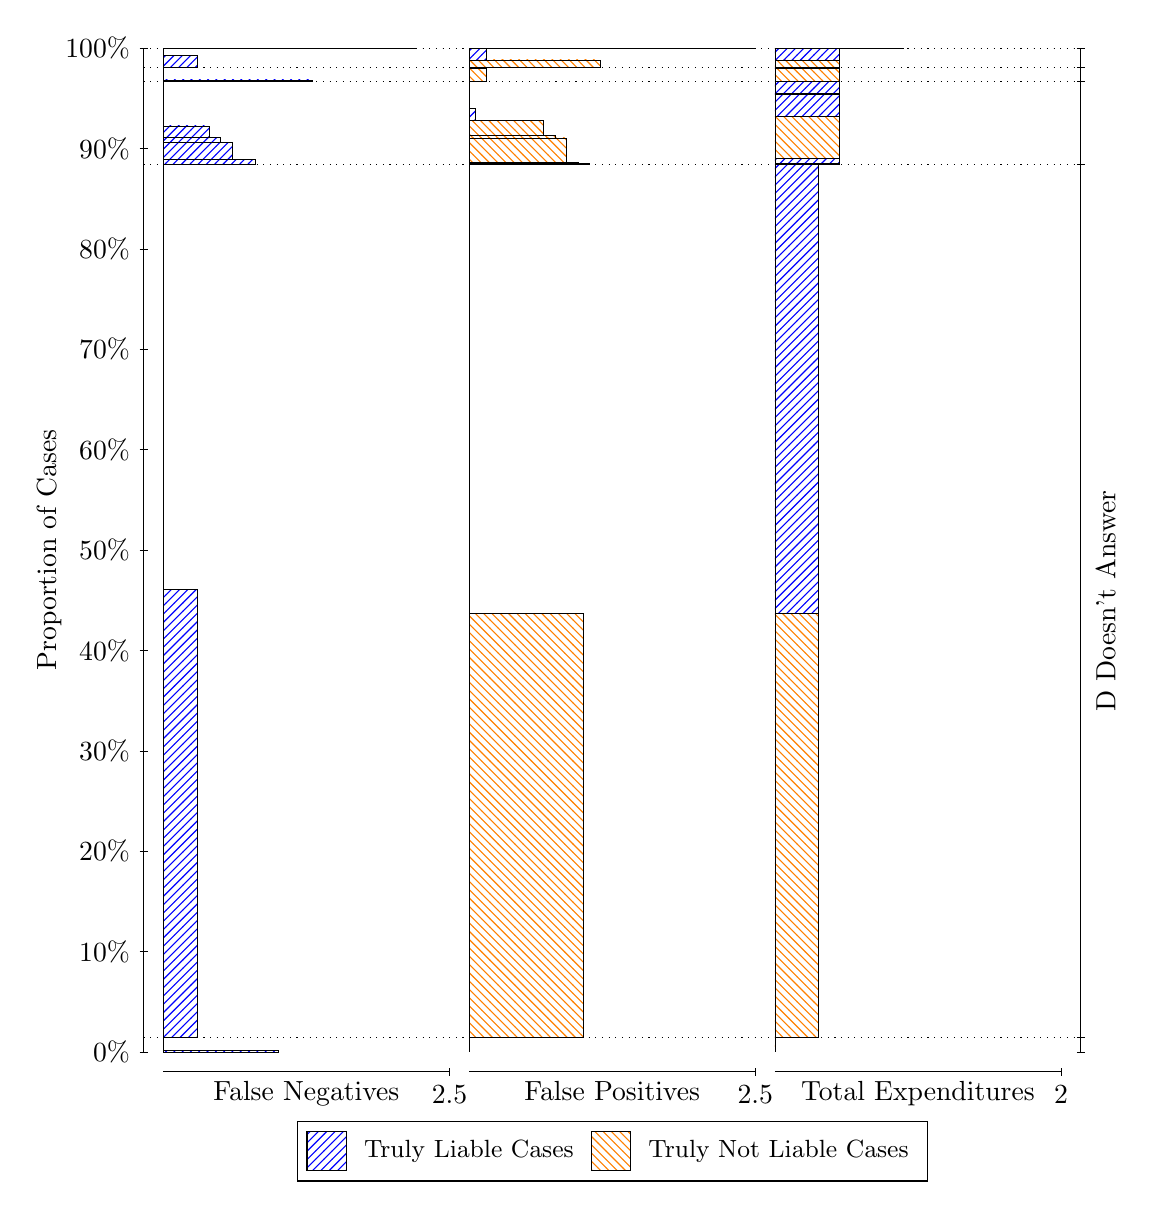
\begin{tikzpicture}
\draw[black, very thin] (1.5,1.75) -- (1.5,14.5);
\node[rotate=90, text=black, anchor=center] at (0.3, 8.125) {Proportion of Cases};
\draw[black, very thin] (1.45,1.75) -- (1.55,1.75);
\node[text=black, anchor=east] at (1.45, 1.75) {0\%};
\draw[black, very thin] (1.45,3.025) -- (1.55,3.025);
\node[text=black, anchor=east] at (1.45, 3.025) {10\%};
\draw[black, very thin] (1.45,4.3) -- (1.55,4.3);
\node[text=black, anchor=east] at (1.45, 4.3) {20\%};
\draw[black, very thin] (1.45,5.575) -- (1.55,5.575);
\node[text=black, anchor=east] at (1.45, 5.575) {30\%};
\draw[black, very thin] (1.45,6.85) -- (1.55,6.85);
\node[text=black, anchor=east] at (1.45, 6.85) {40\%};
\draw[black, very thin] (1.45,8.125) -- (1.55,8.125);
\node[text=black, anchor=east] at (1.45, 8.125) {50\%};
\draw[black, very thin] (1.45,9.4) -- (1.55,9.4);
\node[text=black, anchor=east] at (1.45, 9.4) {60\%};
\draw[black, very thin] (1.45,10.675) -- (1.55,10.675);
\node[text=black, anchor=east] at (1.45, 10.675) {70\%};
\draw[black, very thin] (1.45,11.95) -- (1.55,11.95);
\node[text=black, anchor=east] at (1.45, 11.95) {80\%};
\draw[black, very thin] (1.45,13.225) -- (1.55,13.225);
\node[text=black, anchor=east] at (1.45, 13.225) {90\%};
\draw[black, very thin] (1.45,14.5) -- (1.55,14.5);
\node[text=black, anchor=east] at (1.45, 14.5) {100\%};

\draw[black, very thin] (13.4,1.75) -- (13.4,14.5);
\draw[black, very thin] (13.35,1.75) -- (13.45,1.75);
\node[anchor=west] at (13.35, 1.75) {};
\draw[black, very thin] (13.35,1.9311) -- (13.45,1.9311);
\node[anchor=west] at (13.35, 1.9311) {};
\draw[black, very thin] (13.35,13.021) -- (13.45,13.021);
\node[anchor=west] at (13.35, 13.021) {};
\draw[black, very thin] (13.35,14.075) -- (13.45,14.075);
\node[anchor=west] at (13.35, 14.075) {};
\draw[black, very thin] (13.35,14.258) -- (13.45,14.258);
\node[anchor=west] at (13.35, 14.258) {};
\draw[black, very thin] (13.35,14.493) -- (13.45,14.493);
\node[anchor=west] at (13.35, 14.493) {};
\draw[black, very thin] (13.35,14.498) -- (13.45,14.498);
\node[anchor=west] at (13.35, 14.498) {};
\draw[black, very thin] (13.35,14.5) -- (13.45,14.5);
\node[anchor=west] at (13.35, 14.5) {};

\draw[black, very thin, pattern color=blue, pattern=north east lines] (1.75,1.75) rectangle (3.2033,1.7691);
\draw[black, very thin, pattern color=orange, pattern=north west lines] (1.75,1.7691) rectangle (1.75,1.9311);
\draw[black, very thin, pattern color=blue, pattern=north east lines] (1.75,1.9311) rectangle (2.186,7.6293);
\draw[black, very thin, pattern color=orange, pattern=north west lines] (1.75,7.6293) rectangle (1.75,13.021);
\draw[black, very thin, pattern color=blue, pattern=north east lines] (1.75,13.021) rectangle (2.9127,13.083);
\draw[black, very thin, pattern color=blue, pattern=north east lines] (1.75,13.083) rectangle (2.7673,13.085);
\draw[black, very thin, pattern color=blue, pattern=north east lines] (1.75,13.085) rectangle (2.622,13.299);
\draw[black, very thin, pattern color=blue, pattern=north east lines] (1.75,13.299) rectangle (2.4767,13.365);
\draw[black, very thin, pattern color=blue, pattern=north east lines] (1.75,13.365) rectangle (2.3313,13.512);
\draw[black, very thin, pattern color=orange, pattern=north west lines] (1.75,13.512) rectangle (1.75,14.075);
\draw[black, very thin, pattern color=blue, pattern=north east lines] (1.75,14.075) rectangle (3.6393,14.096);
\draw[black, very thin, pattern color=orange, pattern=north west lines] (1.75,14.096) rectangle (1.75,14.258);
\draw[black, very thin, pattern color=blue, pattern=north east lines] (1.75,14.258) rectangle (2.186,14.402);
\draw[black, very thin, pattern color=orange, pattern=north west lines] (1.75,14.402) rectangle (1.75,14.493);
\draw[black, very thin, pattern color=blue, pattern=north east lines] (1.75,14.493) rectangle (4.9473,14.494);
\draw[black, very thin, pattern color=orange, pattern=north west lines] (1.75,14.494) rectangle (1.75,14.498);
\draw[black, very thin, pattern color=orange, pattern=north west lines] (1.75,14.498) rectangle (1.75,14.499);
\draw[black, very thin, pattern color=blue, pattern=north east lines] (1.75,14.499) rectangle (1.75,14.5);
\draw[black, very thin, pattern color=orange, pattern=north west lines] (5.6333,1.75) rectangle (5.6333,1.912);
\draw[black, very thin, pattern color=blue, pattern=north east lines] (5.6333,1.912) rectangle (5.6333,1.9311);
\draw[black, very thin, pattern color=orange, pattern=north west lines] (5.6333,1.9311) rectangle (7.0867,7.3233);
\draw[black, very thin, pattern color=blue, pattern=north east lines] (5.6333,7.3233) rectangle (5.6333,13.021);
\draw[black, very thin, pattern color=orange, pattern=north west lines] (5.6333,13.021) rectangle (7.1593,13.039);
\draw[black, very thin, pattern color=orange, pattern=north west lines] (5.6333,13.039) rectangle (7.014,13.05);
\draw[black, very thin, pattern color=orange, pattern=north west lines] (5.6333,13.05) rectangle (6.8687,13.359);
\draw[black, very thin, pattern color=orange, pattern=north west lines] (5.6333,13.359) rectangle (6.7233,13.387);
\draw[black, very thin, pattern color=orange, pattern=north west lines] (5.6333,13.387) rectangle (6.578,13.585);
\draw[black, very thin, pattern color=blue, pattern=north east lines] (5.6333,13.585) rectangle (5.706,13.732);
\draw[black, very thin, pattern color=blue, pattern=north east lines] (5.6333,13.732) rectangle (5.6333,14.075);
\draw[black, very thin, pattern color=orange, pattern=north west lines] (5.6333,14.075) rectangle (5.8513,14.238);
\draw[black, very thin, pattern color=blue, pattern=north east lines] (5.6333,14.238) rectangle (5.6333,14.258);
\draw[black, very thin, pattern color=orange, pattern=north west lines] (5.6333,14.258) rectangle (7.3047,14.348);
\draw[black, very thin, pattern color=blue, pattern=north east lines] (5.6333,14.348) rectangle (5.8513,14.493);
\draw[black, very thin, pattern color=orange, pattern=north west lines] (5.6333,14.493) rectangle (5.6333,14.496);
\draw[black, very thin, pattern color=blue, pattern=north east lines] (5.6333,14.496) rectangle (5.6333,14.498);
\draw[black, very thin, pattern color=orange, pattern=north west lines] (5.6333,14.498) rectangle (9.2667,14.499);
\draw[black, very thin, pattern color=blue, pattern=north east lines] (5.6333,14.499) rectangle (7.8133,14.5);
\draw[black, very thin, pattern color=orange, pattern=north west lines] (9.5167,1.75) rectangle (9.5167,1.912);
\draw[black, very thin, pattern color=blue, pattern=north east lines] (9.5167,1.912) rectangle (9.5167,1.9311);
\draw[black, very thin, pattern color=orange, pattern=north west lines] (9.5167,1.9311) rectangle (10.062,7.3233);
\draw[black, very thin, pattern color=blue, pattern=north east lines] (9.5167,7.3233) rectangle (10.062,13.021);
\draw[black, very thin, pattern color=orange, pattern=north west lines] (9.5167,13.021) rectangle (10.334,13.032);
\draw[black, very thin, pattern color=blue, pattern=north east lines] (9.5167,13.032) rectangle (10.334,13.098);
\draw[black, very thin, pattern color=orange, pattern=north west lines] (9.5167,13.098) rectangle (10.334,13.633);
\draw[black, very thin, pattern color=blue, pattern=north east lines] (9.5167,13.633) rectangle (10.334,13.91);
\draw[black, very thin, pattern color=orange, pattern=north west lines] (9.5167,13.91) rectangle (10.334,13.928);
\draw[black, very thin, pattern color=blue, pattern=north east lines] (9.5167,13.928) rectangle (10.334,14.075);
\draw[black, very thin, pattern color=orange, pattern=north west lines] (9.5167,14.075) rectangle (10.334,14.238);
\draw[black, very thin, pattern color=blue, pattern=north east lines] (9.5167,14.238) rectangle (10.334,14.258);
\draw[black, very thin, pattern color=orange, pattern=north west lines] (9.5167,14.258) rectangle (10.334,14.348);
\draw[black, very thin, pattern color=blue, pattern=north east lines] (9.5167,14.348) rectangle (10.334,14.493);
\draw[black, very thin, pattern color=orange, pattern=north west lines] (9.5167,14.493) rectangle (11.152,14.496);
\draw[black, very thin, pattern color=blue, pattern=north east lines] (9.5167,14.496) rectangle (11.152,14.498);
\draw[black, very thin, pattern color=orange, pattern=north west lines] (9.5167,14.498) rectangle (11.152,14.499);
\draw[black, very thin, pattern color=blue, pattern=north east lines] (9.5167,14.499) rectangle (11.152,14.5);
\draw[black, dotted] (1.5,1.9311) -- (13.4,1.9311);
\draw[black, dotted] (1.5,13.021) -- (13.4,13.021);
\draw[black, dotted] (1.5,14.075) -- (13.4,14.075);
\draw[black, dotted] (1.5,14.258) -- (13.4,14.258);
\draw[black, dotted] (1.5,14.493) -- (13.4,14.493);
\draw[black, dotted] (1.5,14.498) -- (13.4,14.498);
\draw[black, very thin] (1.75,1.5) -- (5.3833,1.5);
\node[text=black, anchor=north] at (3.5667, 1.5) {False Negatives};
\draw[black, very thin] (5.3833,1.45) -- (5.3833,1.55);
\node[text=black, anchor=north] at (5.3833, 1.45) {2.5};

\draw[black, very thin] (5.6333,1.5) -- (9.2667,1.5);
\node[text=black, anchor=north] at (7.45, 1.5) {False Positives};
\draw[black, very thin] (9.2667,1.45) -- (9.2667,1.55);
\node[text=black, anchor=north] at (9.2667, 1.45) {2.5};

\draw[black, very thin] (9.5167,1.5) -- (13.15,1.5);
\node[text=black, anchor=north] at (11.333, 1.5) {Total Expenditures};
\draw[black, very thin] (13.15,1.45) -- (13.15,1.55);
\node[text=black, anchor=north] at (13.15, 1.45) {2};


\node[text=black, centered, rotate=90] at (13.72, 7.4763) {D Doesn't Answer};






\draw (7.449999999999999,1.5) node[draw=none] (baseCoordinate) {};
\begin{scope}[align=center]
        \matrix[scale=0.5, draw=black, below=0.5cm of baseCoordinate, nodes={draw}, column sep=0.1cm]{
            \node[rectangle, draw, minimum width=0.5cm, minimum height=0.5cm, pattern color=blue, pattern=north east lines] {}; &
            \node[draw=none, font=\small, text=black] (B) {Truly Liable Cases}; &
            \node[rectangle, draw, minimum width=0.5cm, minimum height=0.5cm, pattern color=orange, pattern=north west lines] {}; &
            \node[draw=none, font=\small, text=black] (B) {Truly Not Liable Cases}; \\
            };
\end{scope}

\end{tikzpicture}
\end{document}